\section{Ambiguidade das Regras Oficiais}

Agora que as regras oficiais do jogo foram expostas, podemos analisar com profundidade alguns de seus aspectos e verificar que, na verdade, algumas questões não foram completamente respondidas. Vamos a elas, tentando dirimir as ambiguidades ao comparar as regras em português com a versão original, em inglês\footnote{Disponível na mesma folha que exibe as regras em português, e também \textit{online} no site http://www.mattelgamefinder.com/rules/uno(eng).pdf}.

Caso a ambiguidade não possa ser desfeita, depois de cada uma, uma seção com opções --- escolhas a serem feitas entre um modo de jogar e outro --- será apresentada. Cada opção possui um código para que você possa fazer referência às suas escolhas quanto ao jogo.

\subsection{Procedimentos Pré-jogo}

A regra diz que:

\begin{quotation}
Cada jogador compra uma carta. A pessoa que tirar a carta mais alta faz a distribuição. [...] Quando as cartas estiverem embaralhadas, são distribuídas 7 cartas para cada jogador.

[...] A carta de cima do MONTE é virada para cima para começar uma pilha de DESCARTE. [...] O jogador à esquerda do distribuidor começa o jogo.
\end{quotation}

A questão é que o jogo parece ter tornado mais simples (e bem diferente) a tradição de distruibuição de cartas aplicada a jogos como Truco, Canastra e Caxeta (ou ``Pife'').

Na maioria dos jogos, uma pessoa deve embaralhar as cartas. Depois, o distribuidor em questão deve passar as cartas para o jogador à \textit{esquerda}, que então \textit{corta} as cartas. Durante o corte, este jogador deve pegar uma carta do local onde o corte foi feito e virá-la para a cima --- no caso do Truco ou da Caxeta, esta carta em questão define o \textit{curinga}. No caso do UNO, apenas determina quais cartas poderão ser jogadas pelo jogador que inicia a partida.

Após feito o corte, as duas partes do baralho encontram-se novamente na ordem em que estavam antes, e o distribuidor passa então a distribuir as cartas, começando pelo jogador imediatamente à sua direita e prosseguindo no sentido anti-horário até que dê as suas próprias cartas\footnote{Algumas regras podem ser mais complexas; no Truco, se o jogador que corta escolher a carta de baixo do monte para definir o curinga, o distribuidor deve distribuir as cartas de baixo do monte. Além disso, podem existir regras específicas quanto ao número de cartas dadas aos jogadores a cada volta no sentido anti-horário até que todos os jogadores tenham o número de cartas estipulado para começar o jogo.}. Após isso, o jogador à \textit{direita} inicia o jogo.

Tudo isso parece ter sido apenas subentendido ou ignorado nas regras do UNO; considerando, contudo, que eles não fazem menção alguma à ideia do jogador que faz o corte, e explicitam que o jogo deve começar pela \textit{esquerda}, é mais provável que toda a convenção tenha sido ignorada e o que ocorra seja um procedimento mais simples (até pela natureza comercial, que tende a simplificar as coisas, do jogo): o jogador que tira a carta mais alta faz a distribuição, na ordem que quiser, qualquer um pode virar uma carta do monte para formar a pilha de descarte, e o jogador à esquerda inicia o jogo.

O que a regra não parece clarificar, contudo, é quantas vezes este procedimento precisa ser repetido: apenas no início do \textit{jogo} ou a cada \textit{partida} dentro do mesmo jogo? Considerando que se o procedimento for feito a cada início de partida, a sorte acaba por determinar quem começa o jogo mais vezes. O curso normal do jogo geralmente faz com que a vantagem de começar uma partida em geral seja pequena, mas ainda assim é uma vantagem. Portanto, para maior equilíbrio, seria mais natural fazer com que, uma vez definido quem dá as cartas \textit{na primeira partida do jogo}, os distribuidores sejam escolhidos através de um ciclo no sentido horário (à esquerda), dando assim a todos a chance de embaralhar as cartas e iniciar a partida.

\subsubsection{Opções}

\begin{itemize}
\item{Adotar os procedimentos pré-jogo simplificados do UNO. Código 1.}
\item{Adotar os procedimentos pré-jogo tradicionais. Código 2.}
\item{Adotar os procedimentos pré-jogo simplificados do UNO apenas no começo do jogo, e depois partir para o uso dos tradicionais. Código 3.}
\end{itemize}

\subsection{Correções}

\begin{quote}
Se um jogador jogar uma carta errada e isto for notado por qualquer um dos demais jogadores, ele ``precisa'' pegá-la de volta e comprar mais 2 cartas extras do MONTE. O jogo continua com o próximo jogador.
\end{quote}

\begin{wrapfigure}{i}{0.25\textwidth}
  \begin{center}
    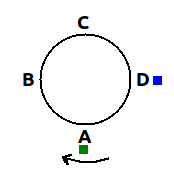
\includegraphics[scale=0.5]{fig1.png}
  \end{center}
  \caption{Se o jogador A faz uma jogada errada (verde), e isso é descoberto apenas na vez do jogador D (azul), após a correção, quem deve jogar? A, B ou D?}
\end{wrapfigure}

As regras não explicam o que ocorre quando o erro é percebido algumas rodadas adiante (mesmo duas ou três). Quem seria ``o próximo jogador''? O próximo, que iria jogar caso o erro não tivesse sido descoberto, ou o jogador que jogou logo após o outro que cometeu o erro? A versão em inglês não elimina a dúvida\footnote{``If a player plays a wrong card and it is noticed by any of the other players, he/she \emph{must} take the card back and take 2 extra cards from the DRAW pile. Play continues with the next person in turn''.}.

Além disso, que tipo de correção deve ser feita ao erro? O jogador que o cometeu deve pegar a carta de volta, comprar duas cartas e jogar alguma outra, desta vez apropriada? Ou deveria apenas pegar sua carta de volta, comprar mais duas e o jogo continua sem a participação desse jogador?

Tudo isto parece uma decisão que se relaciona mais ao valor que se tem em relação ao jogo: o que é mais priorizado? Que o jogo seja justo, correto, ou que seja mais rápido e dinâmico? Este é um tipo de decisão (dentre outras) que se encontra no cerne de praticamente todas as variações e personalizações do jogo contidas neste guia.

Suponha que você esteja jogando dentro de um sistema de apostas. É primordial, assim, que o jogo seja o mais justo possível; logo, o que deve ser feito é uma correção imediata e o jogo deve reiniciar a partir do primeiro jogador afetado, que precisa refazer a sua jogada.

Contudo, alguns jogadores podem ter se beneficiado do erro alheio, e para que o jogo não seja totalmente refeito, o que se pode fazer é continuar o jogo normalmente, mas com o jogador que errou comprando duas cartas e recebendo suas cartas da jogada equivocada de volta.

Há um ponto em comum, contanto: erros causam consternação, dúvida, problemas de estratégia não-necessários. Puni-los para não incentivá-los é uma prática razoável; não faz sentido, pois, que o jogador tenha chance de jogar outras cartas (desta vez, corretas) caso tenha errado. Ainda assim, é uma opção.

\subsubsection{Opções}

\begin{itemize}
\item{O erro é corrigido com o jogador pegando de volta a carta que jogou erroneamente, com a partida reiniciada daquele ponto. Código 1.}
\item{O jogador errado é punido, mas as jogadas subsequentes não são alteradas. A partida prossegue. Código 2.}
\end{itemize}

\subsection{O Desafio do Curinga}

A regra diz:

\begin{quote}
Se um Curinga Comprar Quatro Cartas for exibido indevidamente (isto é, se o jogador possuir uma carta da mesma cor da que está na pilha de DESCARTE) e a pessoa que estiver jogando for desafiada, a mão precisa ser mostrada \textit{primeiro} ao jogador que fez o desafio.
\end{quote}

A ênfase dada ao termo \textit{primeiro} parece sugerir que as cartas devam ser mostradas a todos os jogadores, mas primeiramente para o desafiante --- o que certamente é desnecessariamente prejudicial ao jogador desafiado, uma vez que todos passariam a ver suas cartas, embora apenas uma pessoa já basta para determinar se a jogada foi legítima ou não. A versão em inglês das regras não colabora para o esclarecimento, tampouco\footnote{``If a Wild Draw Four card is played illegally (that is, if the player holds a matching color to one that’s on the DISCARD pile) and the person who plays it is challenged, the hand must \emph{first} be shown to the player who has made the challenge''.}.

\subsubsection{Opções}

\begin{itemize}
\item{O jogador desafiado deve mostrar as suas cartas a todos. Código 1.}
\item{O jogador desafiado deve mostrar suas cartas apenas ao desafiante. Código 2.}
\end{itemize} 

\textbf{Além disso}, se um blefe for descoberto, a carta jogada ainda é válida? O jogador que a jogou ainda tem, pelo menos, o direito de exigir a cor? Me parece um modo de não tornar o blefe uma ação muito arriscada, estimulando-a e tornando o jogo mais divertido e complexo.

\subsubsection{Opções}

\begin{itemize}
\item{Se o blefe for descoberto, o desafiado pelo menos exige uma cor. Código 1.}
\item{Se o blefe for descoberto, a carta torna-se inválida. Código 2.}
\end{itemize}

\subsection{A Cor do Descarte}

A regra diz o seguinte:

\begin{quote}
[...] Esta carta \textit{[Curinga Comprar Quatro Cartas]} só pode ser jogada quando o jogador que a possui não tiver na mão uma carta de mesma cor da que está na pilha de DESCARTE.
\end{quote}

Esta é curiosa, e até mesmo filosófica: suponhamos que um jogador jogue esta carta. O próximo deve comprar quatro, e perde a vez. O jogador que a jogou escolhe a próxima cor: amarelo. O jogador que vai jogar agora possui uma carta amarela, mas possui também um Curinga Comprar Quatro Cartas.

Teoricamente, a \textit{carta que está pilha de DESCARTE} não tem cor. Ou poderíamos dizer que ela é ``preta'', por ser um Curinga. Nesse caso, você tem uma carta da mesma cor (o Curinga) pra jogar, e portanto deve jogar esta carta --- o que é redundante, porque esta carta é o Curinga.

Contudo, não faz sentido considerar os Curingas como sendo de uma cor própria; eles assumem cores diferentes. Se o jogador anterior exigiu a cor amarela, o Curinga deve ser tratado como uma carta amarela. Dessa forma, a pessoa tem uma carta amarela pra jogar e ``não pode'' (i.e a não ser que blefe) jogar o Curinga Comprar Quatro Cartas.

\subsection{Fim das Cartas}

A regra diz que:

\begin{quote}
Se nenhum jogador estiver sem cartas quando o MONTE acabar, o baralho é novamente embaralhado e o jogo continua.
\end{quote}

Implica-se, de boa fé, que as instruções na verdade sejam ``Se nenhum jogador estiver sem cartas quando o MONTE acabar, o DESCARTE é novamente embaralhado e a \textit{partida} continua.'', mas boa fé não é necessária, pois a versão inglesa não deixa dúvidas. Uma vez que, no início das regras, tenha sido dito que ``The person to the left of the dealer starts play'' (A pessoa à esquerda começa a \emph{partida}), a frase posterior, ``[...] the deck is reshuffled and play continues'', quer dizer que a \emph{partida} continua.

\subsection{Desafio UNO}

Esta é, na verdade, a ambiguidade que melhor poderemos eliminar com o auxílio da versão inglesa das regras oficiais. Segundo as regras em português, o Desafio UNO é uma variação oficial do jogo. A regra explica:

\begin{quote}
Este jogo é pontuado mantendo-se um total parcial das cartas que estão na mão de cada jogador. Quando um jogador alcança um valor combinado, possivelmente 500, o jogador é eliminado do jogo. Quando restarem apenas dois jogadores, eles jogam de igual pra igual. O jogador que alcançar ou superar o valor combinado perde. [...]
\end{quote}

Há um problema com essa variação de jogo: como exatamente se conta os pontos do total \textit{parcial} das cartas? Alguma pessoa, que não está jogando, deve manter um registro de cada jogador? E como é a dinâmica de jogo? Como é possível \textit{alcançar} uma pontuação nas cartas à mão, se a dinâmica de jogo leva o jogador a descartar cartas, não a acumulá-las? 

Ora, é simples: Desafio UNO não existe nas regras em inglês. Na verdade, este último parágrafo todo é um prolongamento das regras para jogos com oito pessoas, feitos em duas mesas. A versão completa e modificada para que o sentido seja mais preciso, ficaria mais ou menos assim:

\begin{quotation}
Com oito jogadores, eles podem ser jogar separadamente em duas mesas e cada jogador tem outro jogador como parceiro durante quatro partidas (um total de 28 partidas). Pontuação como acima.

Este jogo é pontuado mantendo-se uma pontuação das cartas que ficam na mão de cada jogador ao fim de cada partida. Quando um jogador alcança um valor combinado, possivelmente 500, o jogador é eliminado do jogo. Quando restarem apenas dois jogadores, eles jogam um contra o outro. O jogador que alcançar ou superar o valor combinado perde. O ganhador da última partida é declarado o vencedor do jogo (veja regras especiais para JOGO EM DUPLA).
\end{quotation}

\section{Os Próximos Exemplos}

Os próximos exemplos do livro tratarão do UNO em sua variante que considerei a mais direta e mais simples, com as interpretações mais baseadas no bom senso possíveis (se é que isto é possível): a variante \emph{1121}.

O código é lido da seguinte forma: ele possui quatro números porque nesta seção existem 4 seções com opções (com escolhas a fazer sobre o jogo). Os números estão ordenados de acordo com a ordem de aparecimento dessas seções. O primeiro número é 1; a primeira seção é Procedimentos Pré-jogo; ou seja, das duas opções contidas naquela seção, a de código 1 foi escolhida. E assim por diante.

Nesta variação, os procedimentos pré-jogo simplificados do UNO são adotados, as correções são precisas e o jogo todo precisa ser reiniciado, o jogador desafiado deve mostrar suas cartas apenas ao desafiante, e aquele que for pego no blefe pelo menos exige a próxima cor.